\pagebreak


\blankAteven
\pagestyle{empty}
\begingroup
\formular % usar a mesma família dos capítulos
\fontsize{7}{8}\selectfont

\color{black}
% Make italicized titles use the default serif font even inside Formular
\let\oldtextit\textit
\renewcommand{\textit}[1]{{\addfontfeatures{Scale=MatchLowercase}\rmfamily\oldtextit{#1}}}


\IfFileExists{img/hedra_edicoes_branco.png}{%
  \vspace*{3mm}\noindent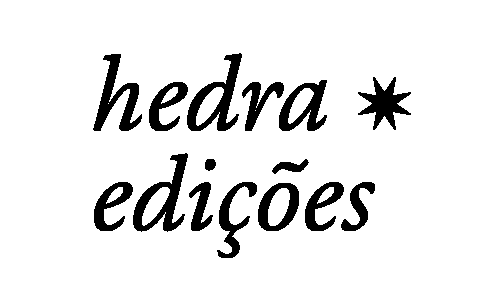
\includegraphics[width=.42\textwidth,keepaspectratio]{img/hedra_edicoes_branco.png}\par
}{%
  \IfFileExists{img/HEDRA_EDICOES_LOGOBRANCO.png}{%
    \vspace*{3mm}\noindent\includegraphics[width=.42\textwidth,keepaspectratio]{img/HEDRA_EDICOES_LOGOBRANCO.png}\par
  }{\large\textsc{hedra edições}}%
}

% Remove the trailing dot after enumerate numbers (local to this group)
\makeatletter
\renewcommand{\labelenumi}{\arabic{enumi}}
\renewcommand{\labelenumii}{\arabic{enumii}}
\renewcommand{\labelenumiii}{\arabic{enumiii}}
\makeatother

\begin{enumerate}
\setlength\parskip{4.2pt}
\setlength\itemsep{-1.4mm}
%\item \textit{Poemas da cabana montanhesa}, Saigy\=o
\item \textit{A arte da guerra}\quad Maquiavel
\item \textit{A conjuração de Catilina}\quad Salústio
\item \textit{A cruzada das crianças\,/\,Vidas imaginárias}\quad Marcel Schwob
\item \textit{A filosofia na era trágica dos gregos}\quad Friedrich Nietzsche
\item \textit{A fábrica de robôs}\quad Karel Tchápek 
\item \textit{A história trágica do Doutor Fausto}\quad Christopher Marlowe
\item \textit{A metamorfose}\quad Franz Kafka
\item \textit{A monadologia e outros textos}\quad Gottfried Leibniz
\item \textit{A morte de Ivan Ilitch}\quad Lev Tolstói 
\item \textit{A velha Izerguil e outros contos}\quad Maksim Górki
\item \textit{A vida é sonho}\quad Calderón de la Barca
\item \textit{A volta do parafuso}\quad Henry James
\item \textit{A voz dos botequins e outros poemas}\quad Paul Verlaine 
\item \textit{A vênus das peles}\quad Leopold von Sacher{}-Masoch
\item \textit{A última folha e outros contos}\quad O.\,Henry
\item \textit{Americanismo e fordismo}\quad Antonio Gramsci
\item \textit{Anarquia pela educação}\quad Élisée Reclus 
\item \textit{Apologia de Galileu}\quad Tommaso Campanella 
\item \textit{Arcana C\oe lestia} e \textit{Apocalipsis revelata}\quad Emanuel Swedenborg
\item \textit{As bacantes}\quad Eurípides
\item \textit{Autobiografia de uma pulga}\quad [Stanislas de Rhodes]
\item \textit{Ação direta e outros escritos}\quad Voltairine de Cleyre
\item \textit{Balada dos enforcados e outros poemas}\quad François Villon
\item \textit{Carmilla, a vampira de Karnstein}\quad Sheridan Le Fanu
\item \textit{Carta sobre a tolerância}\quad John Locke
\item \textit{Contos clássicos de vampiro}, L.\,Byron, B.\,Stoker \& outros
\item \textit{Contos de amor, de loucura e de morte}\quad Horacio Quiroga
\item \textit{Contos indianos}\quad Stéphane Mallarmé
\item \textit{Cultura estética e liberdade}\quad Friedrich von Schiller
\item \textit{Cântico dos cânticos}\quad [Salomão]
\item \textit{Dao De Jing}\quad Lao Zi
\item \textit{Discursos ímpios}\quad Marquês de Sade
\item \textit{Dissertação sobre as paixões}\quad David Hume
\item \textit{Diário de um escritor (1873)}\quad Fiódor Dostoiévski
\item \textit{Diário parisiense e outros escritos}\quad Walter Benjamin
\item \textit{Diários de Adão e Eva}\quad Mark Twain
\item \textit{Don Juan}\quad Molière
\item \textit{Dos novos sistemas na arte}\quad Kazimir Maliévitch
\item \textit{Educação e sociologia}\quad Émile Durkheim
\item \textit{Édipo Rei}\quad Sófocles
\item \textit{Elogio da loucura}\quad Erasmo de Rotterdam
\item \textit{Émile e Sophie ou os solitários}\quad Jean-Jacques Rousseau 
\item \textit{Emília Galotti}\quad Gotthold Ephraim Lessing
\item \textit{Entre camponeses}\quad Errico Malatesta
\item \textit{Ernestine ou o nascimento do amor}\quad Stendhal
\item \textit{Escritos revolucionários}\quad Errico Malatesta
\item \textit{Escritos sobre arte}\quad Charles Baudelaire
\item \textit{Escritos sobre literatura}\quad Sigmund Freud
\item \textit{Eu acuso!}\quad Zola\,/\,\textit{O processo do capitão Dreyfus}, Rui Barbosa
\item \textit{Explosão: romance da etnologia}\quad Hubert Fichte
\item \textit{Fedro}\quad Platão
\item \textit{Feitiço de amor e outros contos}\quad Ludwig Tieck
\item \textit{Flossie, a Vênus de quinze anos}\quad [Swinburne]
\item \textit{Fábula de Polifemo e Galateia e outros poemas}\quad Góngora
\item \textit{Fé e saber}\quad Georg W.\,F.\,Hegel
\item \textit{Gente de Hemsö}\quad August Strindberg 
\item \textit{Hawthorne e seus musgos}\quad Melville
\item \textit{Hino a Afrodite e outros poemas}\quad Safo de Lesbos 
\item \textit{História da anarquia (v.\,\textsc{i})}\quad Max Nettlau
\item \textit{História da anarquia (v.\,\textsc{ii})}\quad Max Nettlau
\item \textit{Imitação de Cristo}\quad Tomás de Kempis
\item \textit{Incidentes da vida de uma escrava}\quad Harriet Jacobs
\item \textit{Inferno}\quad August Strindberg
\item \textit{Investigação sobre o entendimento humano}\quad David Hume
\item \textit{Jazz rural}\quad Mário de Andrade
\item \textit{Jerusalém}\quad William Blake
\item \textit{Joana d'Arc}\quad Jules Michelet
\item \textit{Lira grega}\quad Giuliana Ragusa (org.)
\item \textit{Lisístrata}\quad Aristófanes 
\item \textit{Ludwig Feuerbach e o fim da filosofia clássica alemã}\quad Friederich Engels
\item \textit{Manifesto comunista}\quad Karl Marx e Friederich Engels
\item \textit{Memórias do subsolo}\quad Fiódor Dostoiévski
\item \textit{Metamorfoses}\quad Ovídio
\item \textit{Micromegas e outros contos}\quad Voltaire
\item \textit{Narrativa de William W.\,Brown, escravo fugitivo}\quad William Wells Brown
\item \textit{Nascidos na escravidão: depoimentos norte-americanos}\quad \textsc{wpa}
\item \textit{No coração das trevas}\quad Joseph Conrad
\item \textit{Noites egípcias e outros contos}\quad Aleksandr Púchkin
\item \textit{O casamento do Céu e do Inferno}\quad William Blake
\item \textit{O cego e outros contos}, \textsc{d.\,h}.\,Lawrence
\item \textit{O chamado de Cthulhu}, \textsc{h.\,p.}\,lovecraft
\item \textit{O contador de histórias e outros textos}\quad Walter Benjamin
\item \textit{O corno de si próprio e outros contos}\quad Marquês de Sade
\item \textit{O destino do erudito}\quad Johann Fichte
\item \textit{O estranho caso do dr.\,Jekyll e Mr. Hyde}\quad Robert Louis Stevenson
\item \textit{O fim do ciúme e outros contos}\quad Marcel Proust
\item \textit{O indivíduo, a sociedade e o Estado, e outros ensaios}\quad Emma Goldman
\item \textit{O ladrão honesto e outros contos}\quad Fiódor Dostoiévski
\item \textit{O livro de Monelle}\quad Marcel Schwob
\item \textit{O mundo ou tratado da luz}\quad René Descartes
\item \textit{O novo Epicuro: as delícias do sexo}\quad Edward Sellon
\item \textit{O pequeno Zacarias, chamado Cinábrio}\quad \textsc{e.\,t.\,a.}\,Hoffmann
\item \textit{O primeiro Hamlet}\quad William Shakespeare
\item \textit{O princípio anarquista e outros ensaios}\quad Piotr Kropotkin
\item \textit{O princípio do Estado e outros ensaios}\quad Mikhail Bakunin
\item \textit{O príncipe}\quad Maquiavel
\item \textit{O que eu vi, o que nós veremos}\quad Santos-Dumont
\item \textit{O retrato de Dorian Gray}\quad Oscar Wilde
\item \textit{O sobrinho de Rameau}\quad Diderot
\item \textit{Ode ao Vento Oeste e outros poemas}\quad \textsc{p.\,b.}\,Shelley
\item \textit{Ode sobre a melancolia e outros poemas}\quad John Keats
\item \textit{Odisseia}\quad Homero
\item \textit{Oliver Twist}\quad Charles Dickens
\item \textit{Origem do drama barroco}\quad Walter Benjamin
\item \textit{Os sofrimentos do jovem Werther}\quad Goethe
\item \textit{Os sovietes traídos pelos bolcheviques}\quad Rudolf Rocker
\item \textit{Para serem lidas à noite}\quad Ion Minulescu
\item \textit{Pensamento político de Maquiavel}\quad Johann Fichte
\item \textit{Pequeno-burgueses}\quad Maksim Górki
\item \textit{Pequenos poemas em prosa}\quad Charles Baudelaire
\item \textit{Perversão: a forma erótica do ódio}\quad Robert Stoller
\item \textit{Poemas}\quad Lord Byron
\item \textit{Poesia basca: das origens à Guerra Civil} 
\item \textit{Poesia catalã: das origens à Guerra Civil} 
\item \textit{Poesia espanhola: das origens à Guerra Civil} 
\item \textit{Poesia galega: das origens à Guerra Civil} 
\item \textit{Pr\ae terita}\quad John Ruskin
\item \textit{Primeiro livro dos Amores}\quad Ovídio
\item \textit{Rashômon e outros contos}\quad Ryūnosuke Akutagawa
\item \textit{Revolução e liberdade: cartas de 1845 a 1875}\quad Mikhail Bakunin
\item \textit{Robinson Crusoé}\quad Daniel Defoe
\item \textit{Romanceiro cigano}\quad Federico García Lorca
\item \textit{Sagas}\quad August Strindberg
\item \textit{Sobre a amizade e outros diálogos}\quad Jorge Luis Borges e Osvaldo Ferrari
\item \textit{Sobre a filosofia e outros diálogos}\quad Jorge Luis Borges e Osvaldo Ferrari
\item \textit{Sobre a filosofia e seu método (Parerga e paralipomena)}\quad Arthur Schopenhauer 
\item \textit{Sobre a liberdade}\quad Stuart Mill
\item \textit{Sobre a utilidade e a desvantagem da histório para a vida}\quad Friedrich Nietzsche
\item \textit{Sobre a ética (Parerga e paralipomena)}\quad Arthur Schopenhauer 
\item \textit{Sobre anarquismo, sexo e casamento}\quad Emma Goldman
\item \textit{Sobre o riso e a loucura}\quad [Hipócrates]
\item \textit{Sobre os sonhos e outros diálogos}\quad Jorge Luis Borges e Osvaldo Ferrari
\item \textit{Sobre verdade e mentira}\quad Friedrich Nietzsche
\item \textit{Sonetos}\quad William Shakespeare
\item \textit{Sátiras, fábulas, aforismos e profecias}\quad Leonardo da Vinci
\item \textit{Teleny, ou o reverso da medalha}\quad Oscar Wilde
\item \textit{Teogonia}\quad Hesíodo
\item \textit{Trabalhos e dias}\quad Hesíodo
\item \textit{Triunfos}\quad Petrarca
\item \textit{Um anarquista e outros contos}\quad Joseph Conrad
\item \textit{Viagem aos Estados Unidos}\quad Alexis de Tocqueville
\item \textit{Viagem em volta do meu quarto}\quad Xavier de Maistre 
\item \textit{Viagem sentimental}\quad Laurence Sterne
\end{enumerate}

\medskip
\IfFileExists{img/logo_metabiblioteca.png}{%
  \vspace*{3mm}\noindent
\includegraphics[width=.42\textwidth,keepaspectratio]{img/logo_metabiblioteca.png}\par
}{\large\textsc{metabiblioteca}}

\begin{enumerate}
\setlength\parskip{4.2pt}
\setlength\itemsep{-1.4mm}
\item \textit{A carteira de meu tio}\quad Joaquim Manuel de Macedo
\item \textit{A cidade e as serras}\quad Eça de Queirós
\item \textit{A escrava}\quad Maria Firmina dos Reis
\item \textit{A família Medeiros}\quad Júlia Lopes de Almeida 
\item \textit{A pele do lobo e outras peças}\quad Artur Azevedo
\item \textit{Auto da barca do inferno}\quad Gil Vicente
\item \textit{Bom crioulo}\quad Adolfo Caminha
\item \textit{Cartas a favor da escravidão}\quad José de Alencar
\item \textit{Contos e novelas}\quad Júlia Lopes de Almeida
\item \textit{Crime}\quad Luiz Gama
\item \textit{Democracia}\quad Luiz Gama
\item \textit{Direito}\quad Luiz Gama
\item \textit{Elixir do pajé: poemas de humor, sátira e escatologia}\quad Bernardo Guimarães
\item \textit{Eu}\quad Augusto dos Anjos
\item \textit{Farsa de Inês Pereira}\quad Gil Vicente
\item \textit{Helianto}\quad Orides Fontela
\item \textit{História da província Santa Cruz}\quad Gandavo
\item \textit{Iracema}\quad José de Alencar
\item \textit{Liberdade}\quad Luiz Gama
\item \textit{Mensagem}\quad Fernando Pessoa
\item \textit{Meridiano 55}\quad Flávio de Carvalho
\item \textit{O Ateneu}\quad Raul Pompeia
\item \textit{O cortiço}\quad Aluísio Azevedo
\item \textit{O desertor}\quad Silva Alvarenga
\item \textit{Oração aos moços}\quad Rui Barbosa
\item \textit{Pai contra mãe e outros contos}\quad Machado de Assis
\item \textit{Poemas completos de Alberto Caeiro}\quad Fernando Pessoa
\item \textit{Teatro de êxtase}\quad Fernando Pessoa
\item \textit{Transposição}\quad Orides Fontela
\item \textit{Tratado descritivo do Brasil em 1587}\quad Gabriel Soares de Sousa
\item \textit{Tratados da terra e gente do Brasil}\quad Fernão Cardim 
\item \textit{Utopia Brasil}\quad Darcy Ribeiro
\item \textit{Índice das coisas mais notáveis}\quad Antônio Vieira
\end{enumerate}

\medskip
\IfFileExists{img/HEDRA_QUE_HORAS_SAO_LOGOBRANCO.png}{%
  \vspace*{3mm}\noindent
\includegraphics[width=.42\textwidth,keepaspectratio]{img/HEDRA_QUE_HORAS_SAO_LOGOBRANCO.png}\par
}{\large\textsc{que horas são?}}

\begin{enumerate}
\setlength\parskip{4.2pt}
\setlength\itemsep{-1.4mm}
\item \textit{8/1: A rebelião dos manés}\quad Pedro Fiori Arantes, Fernando Frias e Maria Luiza Meneses
\item \textit{A linguagem fascista}\quad Carlos Piovezani \& Emilio Gentile
\item \textit{A sociedade de controle}\quad J.\,Souza; R.\,Avelino; S.\,Amadeu (org.)
\item \textit{Ativismo digital hoje}\quad R.\,Segurado; C.\,Penteado; S.\,Amadeu (org.)
\item \textit{Crédito à morte}\quad Anselm Jappe
\item \textit{Descobrindo o Islã no Brasil}\quad Karla Lima
\item \textit{Desinformação e democracia}\quad Rosemary Segurado
\item \textit{Dilma Rousseff e o ódio político}\quad Tales Ab'Sáber
\item \textit{Labirintos do fascismo} (v.\,\textsc{i})\quad João Bernardo
\item \textit{Labirintos do fascismo} (v.\,\textsc{ii})\quad João Bernardo
\item \textit{Labirintos do fascismo} (v.\,\textsc{iii})\quad João Bernardo
\item \textit{Labirintos do fascismo} (v.\,\textsc{iv})\quad João Bernardo
\item \textit{Labirintos do fascismo} (v.\,\textsc{v})\quad João Bernardo
\item \textit{Labirintos do fascismo} (v.\,\textsc{vi})\quad João Bernardo
\item \textit{Lugar de negro, lugar de branco?}\quad Douglas Rodrigues Barros
\item \textit{Lulismo, carisma pop e cultura anticrítica}\quad Tales Ab'Sáber
\item \textit{Machismo, racismo, capitalismo identitário}\quad Pablo Polese
\item \textit{Michel Temer e o fascismo comum}\quad Tales Ab'Sáber
\item \textit{O quarto poder: uma outra história}\quad Paulo Henrique Amorim
\item \textit{Universidade, cidade e cidadania}\quad Franklin Leopoldo e Silva
\end{enumerate}

\medskip
\IfFileExists{img/HEDRA_MI_LOGOBRANCO.png}{%
  \vspace*{3mm}\noindent
\includegraphics[width=.42\textwidth,keepaspectratio]{img/HEDRA_MI_LOGOBRANCO.png}\par
}{\large\textsc{mundo indígena}}

\begin{enumerate}
\setlength\parskip{4.2pt}
\setlength\itemsep{-1.4mm}
\item \textit{A folha divina}\quad Timóteo Verá Tupã Popygua
\item \textit{A mulher que virou tatu}\quad Eliane Camargo
\item \textit{A terra uma só}\quad Timóteo Verá Tupã Popygua
\item \textit{A árvore dos cantos}\quad Pajés Parahiteri
\item \textit{Cantos dos animais primordiais}\quad Ava Ñomoandyja Atanásio Teixeira
\item \textit{Crônicas de caça e criação}\quad Uirá Garcia
\item \textit{Círculos de coca e fumaça}\quad Danilo Paiva Ramos
\item \textit{Nas redes guarani}\quad Valéria Macedo \& Dominique Tilkin-Gallois
\item \textit{Não havia mais homens}\quad Luciana Storto
\item \textit{O surgimento da noite}\quad Pajés Parahiteri
\item \textit{O surgimento dos pássaros}\quad Pajés Parahiteri
\item \textit{Os Aruaques}\quad Max Schmidt
\item \textit{Os cantos do homem-sombra}\quad Patience Epps e Danilo Paiva Ramos
\item \textit{Os comedores de terra}\quad Pajés Parahiteri
\item \textit{Xamanismos ameríndios}\quad A.\,Barcelos Neto, L.\,Pérez Gil \& D.\,Paiva Ramos
\end{enumerate}

\medskip
\IfFileExists{img/HEDRA_NARRATIVAS_LOGOBRANCO.png}{%
  \vspace*{3mm}\noindent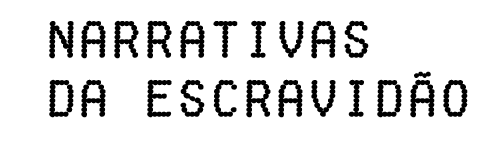
\includegraphics[width=.42\textwidth,keepaspectratio]{img/HEDRA_NARRATIVAS_LOGOBRANCO.png}\par
}{\large\textsc{narrativas da escravidão}}

\begin{enumerate}
\setlength\parskip{4.2pt}
\setlength\itemsep{-1.4mm}
\item \textit{Incidentes da vida de uma escrava}\quad Harriet Jacobs
\item \textit{Nascidos na escravidão: depoimentos norte-americanos}\\quad \textsc{wpa}
\item \textit{Narrativa de William W. Brown, escravo fugitivo}\\quad William Wells Brown
\end{enumerate}

\medskip
\IfFileExists{img/HEDRA_ANARC_LOGOBRANCO.png}{%
  \vspace*{3mm}\noindent\includegraphics[width=.42\textwidth,keepaspectratio]{img/HEDRA_ANARC_LOGOBRANCO.png}\par
}{\large\textsc{anarc}}

\begin{enumerate}
\setlength\parskip{4.2pt}
\setlength\itemsep{-1.4mm}
\item \textit{Sobre anarquismo, sexo e casamento}\\quad Emma Goldman
\item \textit{Ação direta}\\quad Voltairine de Cleyre
\item \textit{O indivíduo, a sociedade e o Estado, e outros ensaios}\\quad Emma Goldman
\item \textit{O princípio anarquista e outros ensaios}\\quad Kropotkin
\item \textit{Os sovietes traídos pelos bolcheviques}\\quad Rocker
\item \textit{Escritos revolucionários}\\quad Malatesta
\item \textit{O princípio do Estado e outros ensaios}\\quad Bakunin
\item \textit{História da anarquia (vol.~1)}\\quad Max Nettlau
\item \textit{História da anarquia (vol.~2)}\\quad Max Nettlau
\item \textit{Entre camponeses}\\quad Malatesta
\item \textit{Revolução e liberdade: cartas de 1845 a 1875}\\quad Bakunin
\item \textit{Anarquia pela educação}\\quad Élisée Reclus 
\end{enumerate}

\medskip
\IfFileExists{img/HEDRA_ECOPOLITICA_LOGOBRANCO.png}{%
  \vspace*{3mm}\noindent
\includegraphics[width=.42\textwidth,keepaspectratio]{img/HEDRA_ECOPOLITICA_LOGOBRANCO.png}\par
}{\large\textsc{ecopolítica}}

\begin{enumerate}
\setlength\parskip{4.2pt}
\setlength\itemsep{-1.4mm}
\item \textit{Anarquistas na América do Sul}\\quad E.\,Passetti, S.\,Gallo; A.\,Augusto  (org.)
\item \textit{Ecopolítica}\\quad E.\,Passetti; A.\,Augusto; B.\,Carneiro; S.\,Oliveira, T.\,Rodrigues  (org.)
\item \textit{Pandemia e anarquia}\\quad E.\,Passetti; J.\,da Mata; J.\,Ferreira  (org.)
\end{enumerate}

% \medskip
% {\large\textsc{coleção <<anarc>>}}

% \begin{enumerate}
% \setlength\parskip{4.2pt}
% \setlength\itemsep{-1.4mm}
% \item \textit{Anarquia pela educação}, Élisée Reclus 
% \item \textit{Ação direta e outros escritos}, Voltairine de Cleyre
% \item \textit{Entre camponeses}, Errico Malatesta
% \item \textit{Escritos revolucionários}, Errico Malatesta
% \item \textit{História da anarquia (vol.\,\textsc{ii})}, Max Nettlau
% \item \textit{História da anarquia (vol.\,\textsc{i})}, Max Nettlau
% \item \textit{O indivíduo, a sociedade e o Estado, e outros ensaios}, Emma Goldman
% \item \textit{O princípio anarquista e outros ensaios}, Piotr Kropotkin
% \item \textit{O princípio do Estado e outros ensaios}, Mikhail Bakunin
% \item \textit{Os sovietes traídos pelos bolcheviques}, Rudolf Rocker
% \item \textit{Revolução e liberdade: cartas de 1845 a 1875}, Mikhail Bakunin
% \item \textit{Sobre anarquismo, sexo e casamento}, Emma Goldman
% \end{enumerate}

% \medskip
% {\large\textsc{coleção <<narrativas da escravidão>>}}

% \begin{enumerate}
% \setlength\parskip{4.2pt}
% \setlength\itemsep{-1.4mm}
% \item \textit{Incidentes da vida de uma escrava}, Harriet Jacobs
% \item \textit{Narrativa de William W.\,Brown, escravo fugitivo}, William Wells Brown
% \item \textit{Nascidos na escravidão: depoimentos norte-americanos}, \textsc{wpa}
% \end{enumerate}

\endgroup % fecha o escopo da fonte Formular
\nopagecolor
\color{black}